\documentclass{article} % For LaTeX2e
\usepackage{nips11submit_e,times}
\usepackage{graphicx}
%\documentstyle[nips10submit_09,times,art10]{article} % For LaTeX 2.09


\title{Perceptual Multistability in a Temporal Illusion}


\author{
Joseph Marrama \\
Department of Symbolic Systems\\
Stanford University\\
\texttt{jmarrama@stanford.edu} \\
\And
Alden Timme \\
Department of Math and Computational Sciences \\
Stanford University \\
\texttt{aotimme@stanford.edu} \\
}

% The \author macro works with any number of authors. There are two commands
% used to separate the names and addresses of multiple authors: \And and \AND.
%
% Using \And between authors leaves it to \LaTeX{} to determine where to break
% the lines. Using \AND forces a linebreak at that point. So, if \LaTeX{}
% puts 3 of 4 authors names on the first line, and the last on the second
% line, try using \AND instead of \And before the third author name.

\newcommand{\fix}{\marginpar{FIX}}
\newcommand{\new}{\marginpar{NEW}}

\nipsfinalcopy % Uncomment for camera-ready version

\begin{document}


\maketitle

\begin{abstract}
In this project, we model the cognitive conception of a visual illusion that can be perceived in four primary modes. 
We model perceptual multistability using a generative Bayesian network that captures the relations between high level features that are extracted from the illusion and the different overall conceptions of the illusion that the viewer can have.
Due to the high complexity of the illusion itself, we simplify the visual stimulus down to a single variable that corresponds to the viewer's observation of the visual stimulus.
Despite this simplifying assumption, our model is sophisticated enough to allow it to exhibit human-like perceptual multistability using Markov Chain Monte Carlo (MCMC) methods to sample from the model conditioned on the observed stimulus.


%In this project, we model the cognitive conception of the reception of a visual field. Our model is a generative Bayesian one in which our uppermost variable represents the viewer’s conception of the visual field – i.e. the background structure of what the viewer sees. Rather than seeing the visual field as a sum of components, the model attempts to express the cognitive phenomenon of interpreting a visual stimulus as a whole cognitive concept. In an illusion, for example, we see one set of components which comprise the entire visual field, but this same set of components can yield multiple interpretations. Viewing this interpretive practice as a Bayesian model, we place the interpretation of the scene at the first layer in the hierarchy. This interpretation then provides a probability distribution over the variables at the second layer, which correspond to the perceived characteristics of the observed components that make up the visual stimulus. Finally, the set of all possible visual stimuli make up the third and final layer.
\end{abstract}


%so , how about an outline to start things off?
%i guess we should sorta shape the writeup like a paper, except much more specific on the model and 
%much shorter on the intro BS

%1. a short intro to perceptual multistability? introduce our illusion, etc....

%2. OUR MODEL - the basic structure, simplifying assumptions
%  question - include only the good gamma-distributed model or both??? which is 'more biologically plausable'?

%3. our results..... which mostly consist of switching times..... 
%  ALSO, model setting the clues in the illusion by setting certain illusion-type things to be constant...



\section{Perceptual Multistability}
%What should be our first section? We should probably do the model first..... 
The mental phenomenon of perceptual multistability is a commonly modeled aspect of human cognition, because it is a well-defined and well-measured phenomenon, and it is fairly easy to model simple illusions that give rise to multistability.
However, little research has gone into modeling perceptual multistability in complex illusions, such as those with a temporal component, multiple stable percepts, and complex structure. 
In our project, we aim to model a high-dimensional temporal illusion with 6 stable percepts (which can be found at bit.ly/c3uGK2) and accurately reconstruct the dynamics of perceptual multistability as it naturally arises from the illusion using MCMC sampling. 


\section{Our Model}
%simplifying the illusion itself, our model, simplifying the featureset, then simplifying the illusion 
Due to the high complexity of the illusion, a number of simplifying assumptions have to be made in order to construct a computationally tractable model. Before we constructed our model, we decided to reduce the number of stable percepts in the illusion to 4 instead of 6, because the mirror images of the double helix and wave forms (see the illusion) are very similar, to the point where they are practically interchangable. The difference between the helix, wave, horizontal motion, and bouncing dots percepts is much more significant than the difference between the 2 wave and helix configurations. 

Using this simplification, we constructed a 3-layer generative Bayesian network for our model. Each variable in each layer (except the bottom layer) contains directed edges going from that variable to every variable in the layer immediately below it. The top layer contains 4 'percept' variables, where each variable can take on a value 1 to 4 that corresponds to a different percept of the illusion. The top layer generates the second layer, which contains intermediate 'high-level feature' variables that correspond to different characteristics one might observe. We have five of these variables, which correspond to observed dimensionality (2d or 3d), planar rotation, horizontal velocity, correlation between dots in each column, and number of objects in the illusion. Lastly, the bottom layer captures the observed illusion. For the bottom layer, we model the input of the illusion as a single 'illusion variable', which has two values corresponding to whether the illusion is being observed or not. This is a very large but necessary simplification, because modeling configurations of the dots in the illusion would've taken hundreds of variables and a temporal model. Also, our approach is still wholly valid, because we can encode the configurations of high-level features that are likely to be observed in the illusion in the conditional probability distribution of the bottom-layer variable. For example, if a configuration of high-level features are observed that \emph{don't} correspond to any percept of the illusion (say, rotation and 2-dimensionality were observed), the illusion variable has a near-zero probability of being active, whereas if a configuration of high-level features that correspond to one of the percepts is observed, then the illusion variable has a near-one probability of being active.

%possibly add a section on more justification for our model? - woooorddddd
Our model can be viewed as a cognitive representation of the reception of a visual field. Staying true to the concepts taught in class, our model is a generative model, where each higher level of abstraction generates the lower. The model can be viewed as a small subset of the complete visual system, where we only use levels of abstraction and variables that are relevant for modeling the illusion. To model the stimulus of the illusion, we condense all lower layers of abstraction/visual processing into a single layer of abstraction that represents all possible visual stimuli, and then only include the one variable that represents the stimuli of the illusion. 

\begin{center}
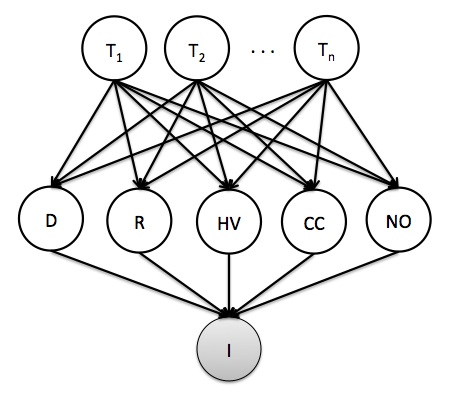
\includegraphics[scale=0.51]{graphical_model}
\end{center}
\small
A graphical representation of our model, with a generalized amount of top-layer percept variables. Our model uses 4 top-layer variables unless stated otherwise.
\normalsize


The CPDs of all the variables in the model can be parameterized as follows. Let the second-layer 'high-level feature' variables be denoted as $\{D, R, HV, CC, NO\}$, where they are in the same order as their enumeration above. Let the top-level percept variables be denoted as $T_1, T_2, T_3, T_4$, the bottom-layer illusion variable as $I$, and finally, let the number of values a variable $U$ can take on be denoted as $|U|$.  

In the illusion, each stable percept corresponds to a unique assignment to the high-level feature variables. Let $c_1$ denote this configuration for viewing the illusion as ovals moving horizontally, $c_2$ the configuration for the double helix, $c_3$ for the wave, and $c_4$ for the dots moving up and down. These are defined as:

\begin{eqnarray*}
c_1 &=& \{D_1,R_1,HV_2,CC_2,NO_2 \} \\
c_2 &=& \{D_2,R_2,HV_1,CC_2,NO_1 \} \\
c_3 &=& \{D_2,R_1,HV_1,CC_2,NO_1 \} \\
c_4 &=& \{D_1,R_1,HV_1,CC_1,NO_3 \} 
\end{eqnarray*}

The probability distributions for all top level variables $T_i$ taking on different percepts is simply distributed according to a multinomial distribution whose parameters are given by a dirichlet distribution with hyper-parameters $\alpha = 200$ (in order to make it give a multinomial distribution close to the uniform distribution) and with a dimension of 4 (because there are 4 possible percepts).
%:
%\begin{eqnarray*}
%P(T_i = j) &=& 0.25 \\
%\end{eqnarray*}

In order to describe the probability distributions for all mid-layer variables $ML$, lets define the following function:
\begin{eqnarray*}
\phi(T_i, ML_x) &=& (1-(|ML|-1)*\epsilon) \textrm{  if } T_i = j \textrm{ and } ML_x \in c_j \\
&=& (\epsilon) \textrm{  if } T_i = j \textrm{ and } ML_x \notin c_j 
\end{eqnarray*}

Now, we can define:

\begin{eqnarray*}
P(ML = x|T_1,T_2,T_3,T_4) &=& \frac{\sum_{i=1}^4 \phi(T_i, ML_x)}{4} 
\end{eqnarray*}

In more understandable terms, the probability $P(ML_x|T_1...T_4)$ is simply the average of all of the contributions of $T_1...T_4$, where the contribution of $T_i$ is simply $(1-\epsilon)$ if $ML_x$ corresponds to the assigned percept of $T_i$, or $\epsilon$ if not. $\epsilon$ can be viewed as a noise term.

Lastly, the CPD for the bottom variable $I$ is:
\begin{eqnarray*}
P(I=1|D,R,HV,CC,NO) &=& (1-\epsilon) \textrm{   if } c_i = \{D,R,HV,CC,NO\} \\
&=& \epsilon \textrm{   if } c_i \neq \{D,R,HV,CC,NO\}  
\end{eqnarray*}


\section{Results}
%how we parameterized the CPDs for the intermediate layer
For all experiments, we used standard Gibbs sampling as our MCMC sampling method, and sampled in order to approximate the posterior $P(M_{-I}|I_1)$, where $I_1$ means the illusion is on and $M_{-I}$ is the whole model sans $I$. Unless otherwise stated, we first sample all variables using forward sampling (and set $I=1$), then use a burn-in time of 10,000 Gibbs samples, and then collect 1,000,000 samples. 
For the experiments discussed below, we use a noise parameter of $\epsilon = 0.01$ and 4 top-level variables $T_i$ unless otherwise stated.  

%FUCK FUCK FUCK stupid fucking shit is hella hard to justify - FMLLLLLLLLL
%As a sanity check to make sure our model is working, we can use the resulting 1,000,000 samples to quickly calculate $P(T_i = j|I = 1)$.


\subsection{Distribution of dominance durations}
As you can see in the figure below, the time to switch between dominant percepts is roughly distributed according to a gamma distribution. We define a 'dominant percept' as anytime 3 or more top-layer percept variables are assigned the same percept. It has been thoroughly documented that switching times in humans between different stable percepts tend to follow a Gamma distribution. Our model has similar behavior. This is likely because each top-layer percept variable has switching times roughly distributed along an exponential distribution, and the Gamma distribution is just a sum of exponential distributions. Nonetheless, our model exhibits human-like characteristics, which is a success of our model. \\

%(insert image and small text beneath it...)
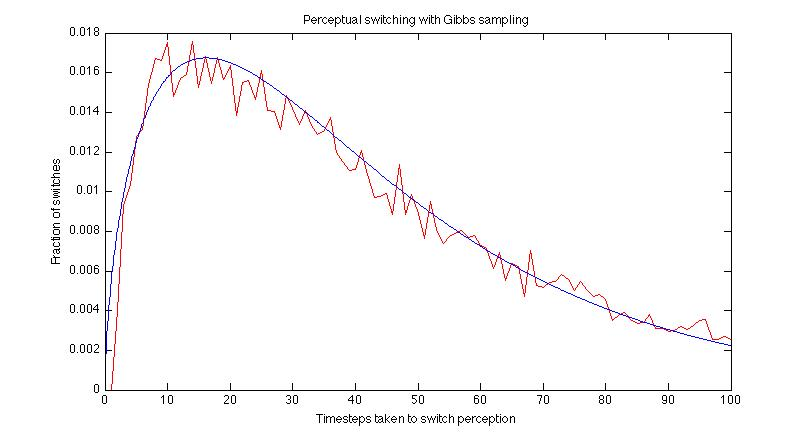
\includegraphics[scale=0.51]{sickbrah}
\small
The percentage of perceptual switches as a function of the timesteps taken to switch percepts is shown in red, and a fitted gamma distribution with a shape parameter of 1.7 and a scale parameter $\Theta = 27$ is shown in blue.
\normalsize


\subsection{Visual Cues}
In the illusion, there are certain visual cues you can set that help you see different percepts. For example, the horizontal motion cue displays a dot moving along with each object to cue the viewer into the fact that there are multiple objects moving along at a high horizontal velocity. This provides a unique opportunity to test our model by holding these cues constant and sampling from the new posterior $P(M_{-I-cues}|I=1, cues)$, and then using the resulting samples to approximate $P(T_i|I=1, cues)$. Intuitively, we should expect $P(T_i = j|I=1, cues)$ to be much higher than $P(T_i = j|I=1)$, assuming the cues are for percept $j$. 

Using the gathered samples from Gibbs sampling on the posterior $P(M_{-I}|I=1)$, we can easily compute the posterior $P(T_i = j|I=1)$ by summing over samples. Computing each $P(T_i = j|I=1)$ and then averaging over all top layer percepts $T_i$, we are left with the following probabilities for $P(T=j|I=1)$: \\ 
.247 for j = Horizontal moving shapes \\
.26 for j = Rotating double helix \\
.24 for j = Wave \\
.253 for j = Uncorrelated bouncing dots \\ 

For the horizontal cue, we decided that the two obvious features the cue prompted the viewer to notice are horizontal motion and multiple objects. Setting $HV = 2$ and $NO = 2$, and using 200,000 iterations of Gibbs sampling to calculate $P(T=j|I=1, HV=2, NO=2)$, we get the following probabilities: \\
.512 for j = Horizontal moving shapes \\
.155 for j = Rotating double helix \\
.153 for j = Wave \\
.168 for j = Uncorrelated bouncing dots \\ 

This is exactly what we would expect to see; observing the cues for Horizontal moving shapes drastically increases the probability of being in that percept. We can do the same for the Helix cue, which tips us off to the features that the illusion is 3-dimensional and rotating. Using 200,000 iterations of Gibbs sampling, $P(T=j|I=1, R=2, D=2)$ = \\
.13 for j = Horizontal moving shapes \\
.472 for j = Rotating double helix \\
.229 for j = Wave \\
.16 for j = Uncorrelated bouncing dots \\ 

Again, this is exactly what we would like to see. Repeating the same process with the other 2 cues leads to similar results; $P(T=j|I,cues)$ is generally around .5 when the cues favor percept $j$. 


\section{Discussion}
Our model differs from some of the other models used for multistability perception (e.g. Gershman 2010) in that it aims to model higher-level cognitive percepts rather than the low-level visual percepts upon which other papers have focused. As a hierarchical generative model of the cognitive formation of the conception of a visual scene, it represents a different approach to modeling perceptual multistability. Many typical lower-level models have been popularized in computer vision for tasks like scene segmentation, such as the pairwise Markov random field (MRF). Despite these different approaches, and subsequently contrasting computational models, both models exhibit some good characteristics that are corroborated by empirical accounts of visual perception of illusions. Namely, both our higher-level hierarchical generative model and the lower-level MRF models exhibit switching times that follow a Gamma-like distribution. This is a well-documented phenomenon of human multistable perception – the amount of time it takes for a human subject to switch perceptions of a multistable illusion is distributed approximately according to a Gamma distribution.

Our model also works well in that it exhibits the correct behavior when one of the particular percepts is highlighted by including cues that reveal high-level features to the viewer. Essentially a visual cue corresponds to observing a subset of the mid-level ‘feature’ variables. With these variables observed to be certain values, Gibbs sampling will favor the mode (i.e. perception) to which the visual cue is most probable. We see the results of clamping variables according to visual cues in the above section.

Despite the good cognitive characteristics of our model, it has some shortcomings that offer various avenues for extension. For one, whereas our model is different from previous models of multistable perception, in principle the two need not be mutually exclusive. In fact, it would make sense to somehow repair the disconnect between a high-level generative cognitive model like ours and lower-level vision models like the pairwise MRF. The ideal model would be one that includes a low-level vision model along with a higher-level one that represents the cognitive interpretation of a visual scene.

The model we use for this project is also specialized to the illusion we are considering. A necessary extension to our modeling idea would be to generalize the model to a wider range of instances of multistable perception and perception in general. One way to do this might be to include a way to learn the set of mid-level features as well as the incoming and outgoing CPDs for the feature variables. Another possible addition to the model would be a larger set of nodes in the final layer, to account for the possibility of viewing different visual fields. Our model considers the scenario in which we have set the visual field to represent the particular illusion we want to model - a more generalized model would probably include a set of visual fields to consider. This is perhaps a good motivation for linking our higher-level cognitive model to a lower-level vision model such as the pairwise MRF.

\section{Conclusion}

We propose a hierarchical generative cognitive model for perceptual multistability. We see from our experiments that it exhibits some of the characteristics of multistable perception in humans. However, our approach is different from past approaches to such models in that it represents a higher-level cognitive interpretation, rather than the low-level models often borrowed from computer vision. In the future, one might try to link the two paradigms into a better hierarchical model that more accurately depicts the process of human vision, from the input and scene segmentation stage to interpretation.











\end{document}
